% ===== Mục 4.2 — Kết quả khối B (≈ 0,5 trang) =====
% Viết gì: bảng E-B1 (không phân lớp, so cổ điển), bảng E-B2 (từng lớp), 2–3 câu nhận xét có số. Người: Trường.
% Nguồn số: results/E-B1/table.csv, results/E-B2/table.csv (hoặc test_metrics.json của notebook train_yolo).
Bảng~\ref{tab:EB} so sánh khả năng tìm vùng chữ khi bỏ qua lớp trong thí nghiệm E-B1 và độ đúng từng lớp của YOLOv8s trong thí nghiệm E-B2.

\begin{table}[H]
\centering
\caption{Phát hiện vùng chữ trên tập kiểm tra, IoU $\ge0{,}5$: nửa trên không phân lớp (E-B1), nửa dưới theo lớp (E-B2).}\label{tab:EB}
\small
\begin{tabular}{lcccc}
\toprule
\textbf{Phương pháp / lớp} & \textbf{P} & \textbf{R} & \textbf{F1} & \textbf{mAP50} \\
\midrule
Cổ điển (Sauvola + giãn) & \num{0.864} & \num{0.776} & \num{0.818} & --- \\
YOLOv8s, bỏ lớp & \textbf{\num{0.991}} & \textbf{\num{0.995}} & \textbf{\num{0.993}} & --- \\
\midrule
\texttt{drugname} & \num{0.998} & \num{1.000} & \num{0.999} & \num{0.995} \\
\texttt{quantity} & \num{1.000} & \num{1.000} & \num{1.000} & \num{0.995} \\
\texttt{usage} & \num{1.000} & \num{0.998} & \num{0.999} & \num{0.995} \\
\texttt{diagnose} & \num{0.996} & \num{0.992} & \num{0.994} & \num{0.993} \\
\texttt{date} & \num{1.000} & \num{1.000} & \num{1.000} & \num{0.995} \\
\texttt{other} & \num{0.987} & \num{0.993} & \num{0.990} & \num{0.995} \\
Cộng dồn mọi vùng & \num{0.991} & \num{0.995} & \num{0.993} & \num{0.995} \\
\bottomrule
\end{tabular}
\end{table}

YOLOv8s tìm vùng chữ tốt hơn rõ rệt, với F1 \num{0.993} so với \num{0.818} của bộ phát hiện cổ điển: bộ cổ điển bỏ sót 1364 trong 6086 vùng và tạo thêm 744 khung thừa, còn YOLOv8s chỉ bỏ sót 30 vùng.
Theo lớp, tên thuốc, số lượng, cách dùng và ngày đạt F1 từ \num{0.999} trở lên; hai lớp yếu hơn là \texttt{other} (\num{0.990}) và \texttt{diagnose} (\num{0.994}).
Ma trận nhầm lẫn ở Hình~\ref{fig:confusion} cho thấy lỗi chủ yếu là bỏ sót 29 vùng \texttt{other} và dự đoán thừa 51 khung \texttt{other}, chỉ 4 vùng bị nhầm sang lớp khác, nên các lớp dùng để ghép khoản gần như không bị ảnh hưởng.

\begin{figure}[H]
\centering
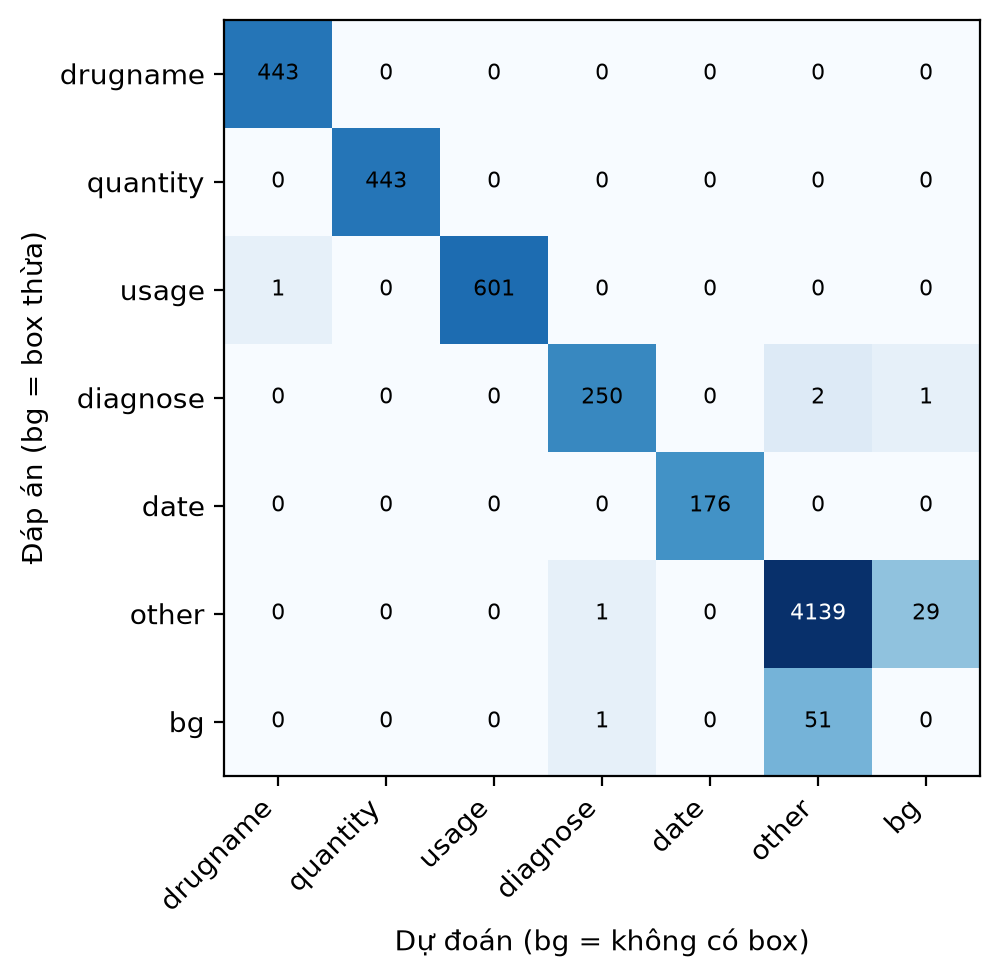
\includegraphics[width=0.42\linewidth]{e_b_detection/b2_confusion.png}
\caption{Ma trận nhầm lẫn của YOLOv8s. Hàng \texttt{bg} là khung thừa, cột \texttt{bg} là vùng bị bỏ sót.}\label{fig:confusion}
\end{figure}